\section{API Gateway}
\subsection{Creazione dell'API Gateway}
Per completare la nostra architettura e disporre di un modo per rispondere in maniera più efficace ed efficiente alle richieste del client abbiamo deciso di creare un API Gateway che facesse da tramite tra il backend scritto in Spring (il ``sistema complesso'') e l'applicazione mobile scritta in Dart. Per fare ciò abbiamo optato per un terzo linguaggio di programmazione, NodeJS, poiché volevamo realizzare un componente che fosse veloce e leggero. Il maggior compito del nostro gateway è quello di interrograre il sistema complesso e comporre le risposte da inviare al client. Grazie al gateway abbiamo riscontrato molti vantaggi mentre lavoravamo all'architettura, tra questi troviamo:
\begin{itemize}
  \item La possibilità di modellare la risposta proveniente dal server in modo da fornire particolari header necessari affinché le risposte fossero accetate dal client. Per esempio includendo l'header `Access-Control-Allow-Origin', richiesto da Dart per accettare una risposta, ma che non era \\ fornito dl sistema complesso;
  \item Permettere a client di ottenere oggetti composti dal sistema complesso che senza l'utilizzo del gateway avrebbero necessitato di numerose chiamate da parte del client. Un esempio è la chiamata di login, la quale, quando l'utente viene autenticato, restituisce informazioni su di esso come nome e cognome. Nella risposta fornita dal Managaer degli Utenti tuttavia non viene fornito il livello di esperirenza. Tuttavia è disponibile una chiamata che soddisfa questa richiesta, dato l'id di un utente. Chiamando questo secondo metodo, dopo aver ottenuto i dati dell'utente, ci ha permesso di includere il campo ``experience'' nella risposta al client.  
\end{itemize}
\newpage
\subsection{Testing del gateway}
Per verificare il corretto funzionamento del gateway abbiamo scritto una serie di test per ognuna delle chiamate verificando che la risposta attesa fosse corretta. Seguono i risultati della test suite (\ref{fig:risTestGateway}).
\begin{figure}[h!]
  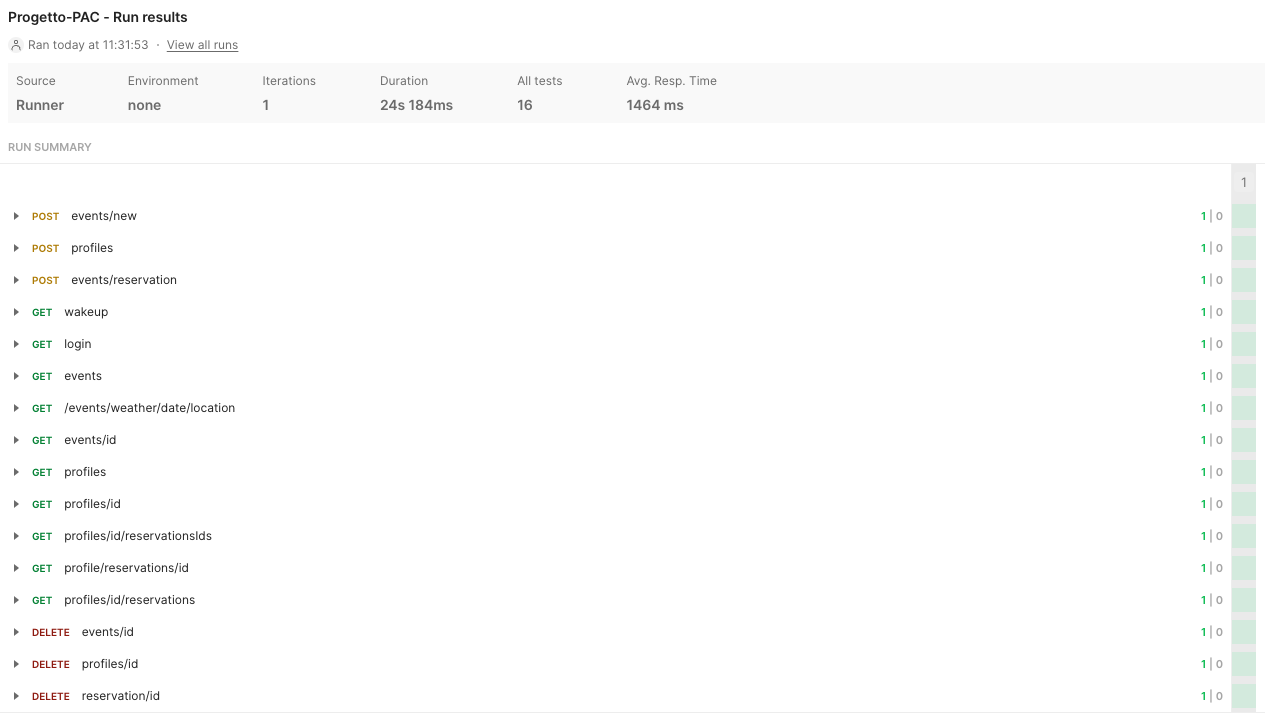
\includegraphics[width=1\textwidth]{Iterazione 3/images/gatewayTest.png}
  \caption{Risultati testing gateway}
  \label{fig:risTestGateway}
\end{figure}